% ----------------------------------------------------------
% Metodologia
% ----------------------------------------------------------
\chapter{Metodologia}\label{cap:metodologia}
% ----------------------------------------------------------
Neste capítulo estão descritos as ferramentas e metodologia utilizadas para o desenvolvimento do projeto, além da apresentação da arquitetura do protótipo de balanceamento proposta. 

% ----------------------------------------------------------
\section{Tecnologias e Ferramentas Utilizadas}\label{sec:tecnologias-ferramentas}
% ----------------------------------------------------------
Nesta seção são apresentadas as ferramentas e tecnologias usadas na implementação do projeto. 

% ---
\subsection{AWS - \textit{Amazon Web Services}}\label{sec:aws}
% ---
A Amazon oferece um vasto portifólio de serviços baseados em Computação em Nuvem, concentrados na Amazon Web Services. Seus produtos variam desde a oferta de IaaS, com servidores virtuais, nuvens privadas, dentre outras ferramentas, até aplicações do tipo SaaS, como o serviço de armazenamento em nuvem (\textit{Amazon Cloud Drive}) \cite{AmazonCloudDrive}.

Sua plataforma de serviços web é centrada no Amazon Elastic Compute Cloud ou EC2. Trata-se de um “serviço que fornece capacidade de computação redimensionável na nuvem” \cite{AmazonEC2}. Por ter foco em desenvolvedores, possui uma interface com maior controle de recursos computacionais, incluindo configurações de memória, processamento, sistema operacional e armazenamento. Além disso, há suporte para outras ferramentas, como banco de dados, \textit{Big Data} e até mesmo Internet das Coisas. Além do baixo custo, uma das vantagens da Amazon está na flexibilidade dos planos de serviços, que são ajustáveis de acordo com a demanda \cite{AmazonEC2price}.

O acesso é feito por meio do AWS Management Console, que consiste em uma interface web para gerenciamento dos serviços. No caso da EC2, a visualização e acompanhamento de estado das instâncias é feito pela EC2 Dashboard, como exemplificado na figura \ref{fig:ec2con}. 

\begin{figure}[htb]
	\caption{\label{fig:ec2con}EC2}
	\begin{center}
		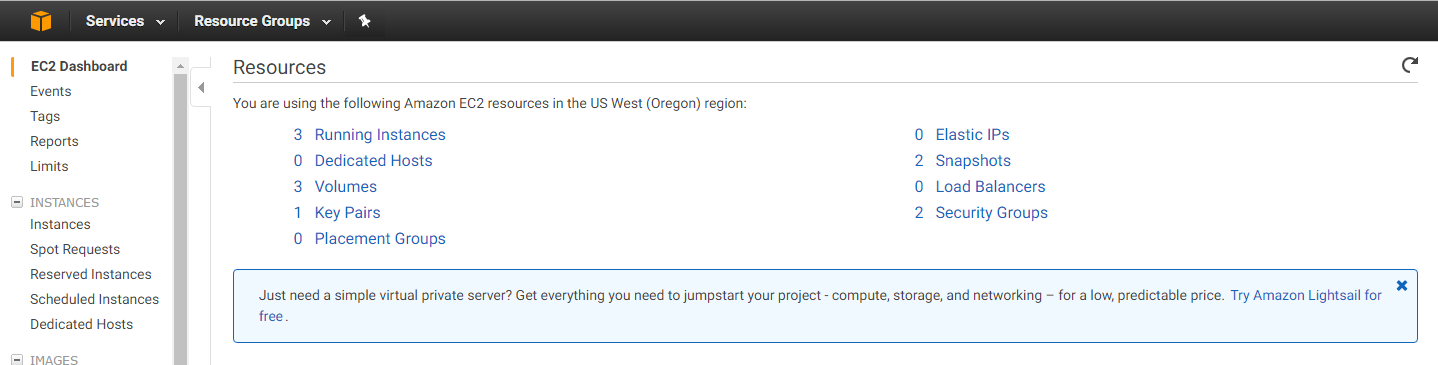
\includegraphics[width=0.90\textwidth]{img/ec2dash.png}
	\end{center}
	\legend{Fonte: elaborada pela autora}
\end{figure}

A AWS oferece diversos tipos de instâncias, as quais os tipos de uso variam de acordo com a aplicação. Instâncias do tipo T2, por exemplo, são indicadas para aplicações web, ambientes de desenvolvimento e teste e preparação de aplicações. Os preços também variam de acordo com o tipo de instância, uso e capacidade computacional \cite{amazon-cloud-instances}.Para este projeto, os servidores utilizados, bem como suas configurações estão descritos na tabela \ref{tab:servidores}. Todos as instâncias possuem como sistema operacional Ubuntu Server 16.04 LTS. 

	\begin{table}[h]
		\caption{Servidores}
		\centering
		\small
		\renewcommand{\arraystretch}{1.2} % Aumenta espaçamento vertical
		\begin{tabular}{c|c|c|c|c}
			\hline 
			\textbf{Servidor} & Tipo de instância & Memória & CPUs & Armazenamento \\ 
			\hline 
			\textbf{Servidor de balanceamento} & t2.medium & 4 & 2 & Somente EBS \\ 
			\hline 
			\textbf{Servidores do \textit{cluster} de aplicação} & t2.micro & 1 & 1 & Somente EBS \\ 
			\hline 
		\end{tabular}\\		
		\vspace{3mm}
		\legend{Elaborado pela autora.}
		\label{tab:servidores}
	\end{table}
	
Os servidores de requisição descritos na tabela \ref{tab:servidores} foram configurados para executar um código semelhante ao apresentado em \ref{sec:node-js} e são acessados apenas pelo servidor de balanceamento, através de seu DNS público, disponibilizado pela AWS para cada instância.  

% ---
\subsection{Node.js e npm}\label{sec:node-js}
% ---

Node.js\footnote{\url{https://nodejs.org/}} é uma plataforma de aplicações baseada no motor de Javascript do Google Chrome chamado V8\cite{nodejs}. Nessa plataforma, o Javascript que geralmente é utilizado no navegador, como forma de tornar dinâmica a interação do lado do cliente, é utilizado como linguagem para fornecer programação direta para o sistema operacional, permitindo a criação e execução no servidor. Seu código fonte está disponível\footnote{\url{https://github.com/nodejs/node}} para acesso, colaboração e comentários.
\begin{figure}[htb]
	\caption{\label{fig:codejs}Código exemplo de servidor em nodejs}
	\begin{center}
		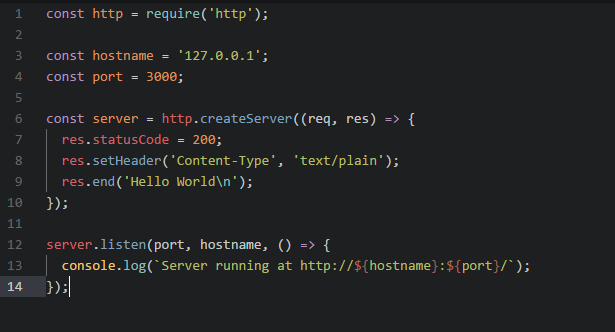
\includegraphics[width=0.90\textwidth]{img/codejs.png}
	\end{center}
	\legend{Fonte: elaborado pela autora}
\end{figure}
Essa plataforma funciona com base em um modelo voltado à eventos, ou seja, a execução não é bloqueada com eventos de entrada e saída (I/O), como nos demais modelos. O Node dispara funções específicas quando os eventos são acionados. Além disso, o Nodejs também possui um gerenciador de pacotes, o \textit{Node Package Manager} (denominado \textit{npm}). Seu objetivo é a instalação e distribuição de pacotes e bibliotecas criadas pela comunidade e que tenham código livre, o que permite que qualquer desenvolvedor disponibilize sua própria biblioteca.

Pacotes criados da maneira descrita anteriormente têm suas informações salvas em um arquivo chamado \textit{packages.json}, o qual contém informações como Nome do projeto, do criador, link para o repositório no GitHub, dependências de bibliotecas com a versão específica instalada, entre outros. Através do comando \textit{npm install} o gerenciador instala as dependências do módulo para executar a aplicação. A plataforma é acessível via terminal de comandos e está disponível para Windows, Mac OS e sistemas operacionais baseados em Linux. Neste projeto, a versão utilizada da plataforma Nodejs foi a 6.6.0. 



A figura \ref{fig:codejs} apresenta um exemplo de código para servidor configurado localmente, na porta 3000. A figura \ref{fig:consolejs} ilustra a execução do código descrito na \ref{fig:codejs} utilizando a plataforma do Nodejs. 

\begin{figure}[htb]
	\caption{\label{fig:consolejs}Exemplo de execução de código em nodejs}
	\begin{center}
		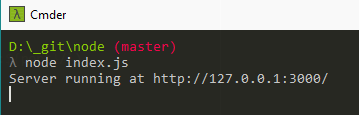
\includegraphics[width=0.90\textwidth]{img/consolejs.png}
	\end{center}
	\legend{Fonte: elaborado pela autora}
\end{figure}
% ---
% ----------------------------------------------------------
\section{Métodos e Etapas}\label{sec:metodos-etapas}
% ----------------------------------------------------------

A primeira fase deste trabalho se concentrou-se no levantamento bibliográfico sobre \textit{Cloud Computing}, balanceamento de carga e Redes Neurais Artificiais. Nesta fase, o estudo se concentrou na pesquisa de serviços de \textit{Cloud} disponíveis no mercado, visto que o teste da ferramenta foi realizado a partir de uma infraestrutura hospedada em uma \textit{Cloud} real. 

A fase seguinte concentrou-se na análise e levantamento das tecnologias utilizadas na implementação da estrutura para testes, inicialmente estudando tecnologias como a ferramenta CloudStack \cite{cloudstack} e a OpenStack \cite{openstack}. Devido à necessidade de possuir uma estrutura de servidores física, ambas as opções citadas foram descartadas e o serviço escolhido foi a EC2\cite{AmazonEC2}, fornecido pela AWS. Durante essa fase, ainda, houve o planejamento e estruturação do módulo que engloba a RNA, bem como sua arquitetura, posteriormente integrada ao módulo de balanceamento de carga. A arquitetura escolhida segue a estrutura descrita pela figura \ref{fig:arq}. 

\begin{figure}[htb]
	\caption{\label{fig:arq}Arquitetura simplificada do projeto}
	\begin{center}
		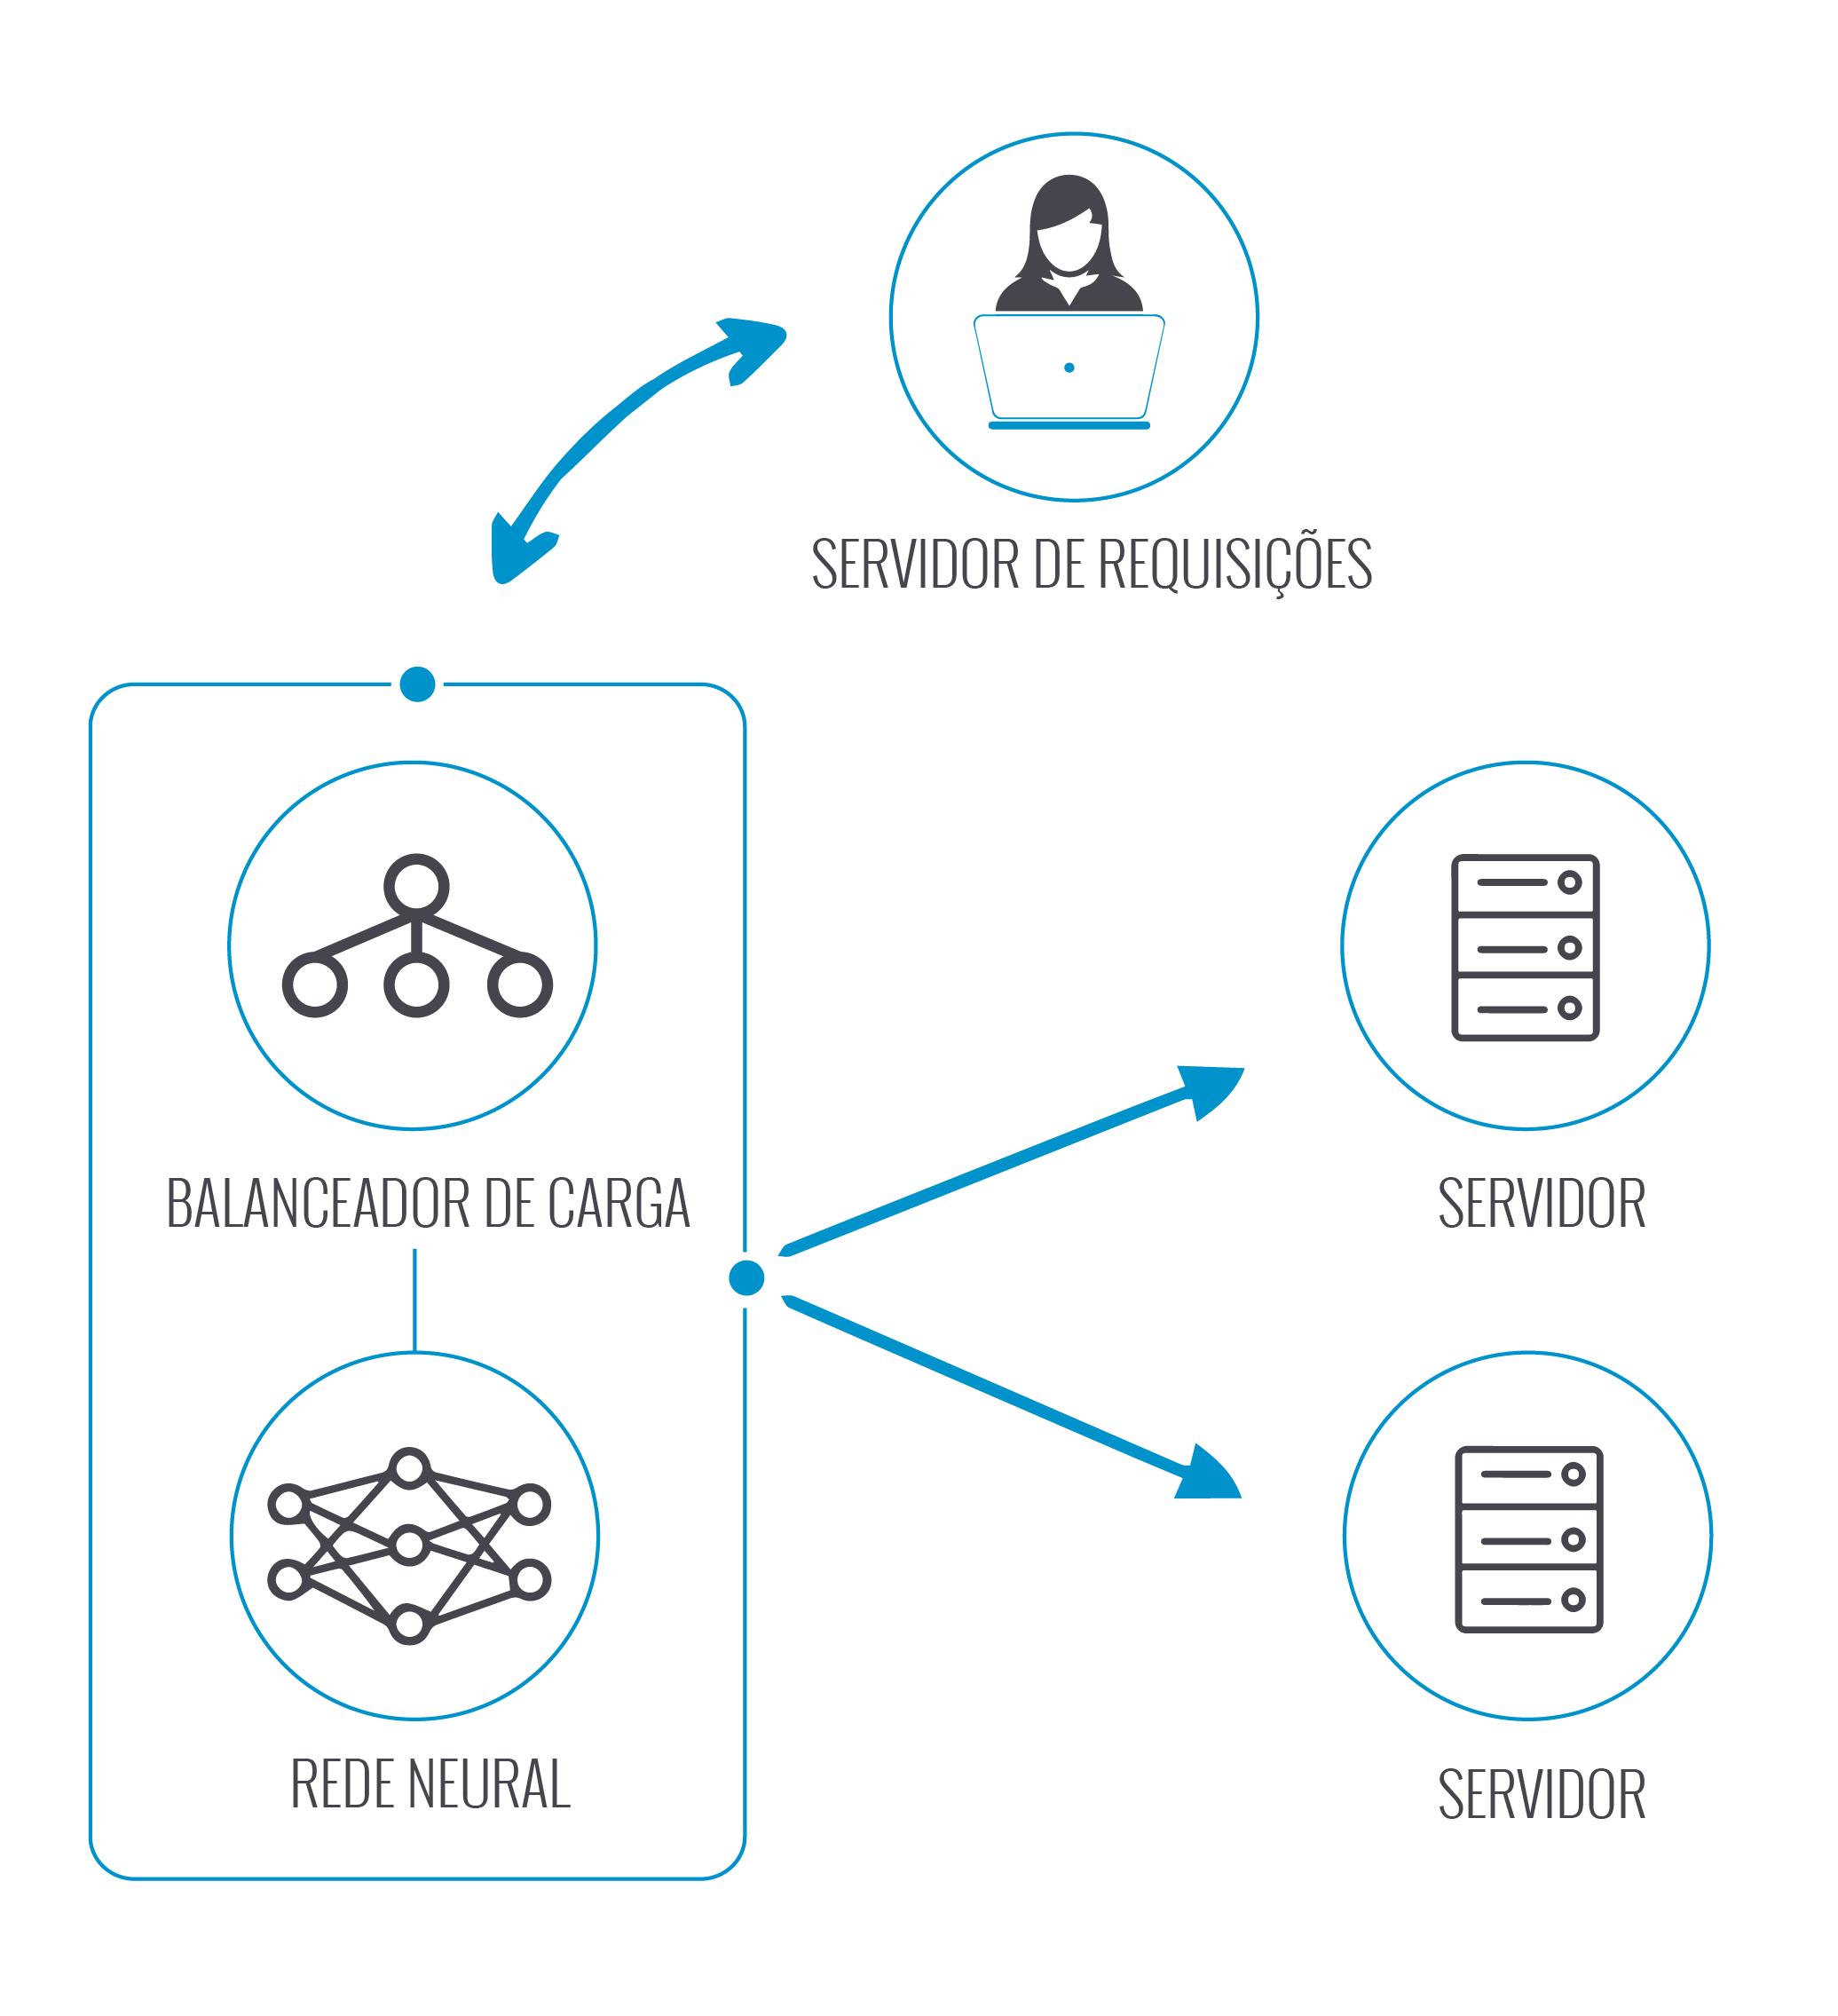
\includegraphics[width=0.50\textwidth]{img/projeto.png}
	\end{center}
	\legend{Fonte: elaborado pela autora}
\end{figure}

A arquitetura do protótipo pode ser dividida em três módulos, como ilustrado na figura \ref{fig:arq}: o primeiro, consiste no servidor responsável pelo balanceamento de carga, o qual recebe todas as requisições que serão posteriormente direcionadas para o \textit{cluster} de servidores de dados; o segundo módulo é composto pelo \textit{cluster} de servidores de dados; e o terceiro é um servidor que gera requisições. Nesta arquitetura, a rede neural é um submódulo do balanceador, sendo responsável pela atribuição de pesos à cada um dos servidores presentes no \textit{cluster} de dados. Estes pesos são utilizados pelo algoritmo de balanceamento para direcionar as requisições aos servidores de modo equilibrado. 

A terceira fase do projeto concentrou-se na implementação e testes do módulo de balanceamento. Nessa fase, o estudo das tecnologias Nodejs e EC2 permitiu a implementação da aplicação e os testes com \textit{clusters} em nuvem.  Essa fase contemplou, ainda, a análise do desempenho da abordagem escolhida, cujo resultado está descrito na seção de Resultados. A fase final do projeto se concentrou na escrita do relatório e apresentação dos resultados obtidos. 
